\documentclass[letterpaper,10pt]{article}
\usepackage{graphicx}

\title{Angular contact with TensorFlow}
\author{Rocco Malisi}

\begin{document}
	\maketitle
	\newpage
	
	\begin{abstract}
		Abstract text here alsdjfsdalsdjlfksdjlk
	\end{abstract}
	\newpage
	
	\tableofcontents
	\newpage
	
	\section{Introduction}
	\section{Methods}
	\section{Results}
	\subsection{Performing an EDA on  angular contact dataset \#1}
	To get a better understanding of dataset \#1, an EDA is performed. The objective is to identify patterns and relationships in the data. The insights gained by this analysis will be used in building and improving the model.
	\newline The dataset consists of three columns and 1365 rows. The columns are 'Fr' (radial force in N[Newton]), 'n' (rotational speed in rpm[revolutions per minute]) and 'Lifetime' (lifetime in h[hours]). The dataset does not contain any empty or null values and therefore does not require cleaning.
	\newline Figure 1 shows a plot of column Fr. The value of Fr starts at 200 and is increased by 100 every 35 rows throughout the whole dataset. The final and highest value of Fr is 4000. 
	\newline The column Lifetime is shown in figure 3. The highest value at the first row is 88445568 but it drops rapidly throughout the dataset to just 116 in the last row. Every 35 rows the value has a local peak but then quickly drops again. Figure 2 is a plot of rows 1000 and up which shows that this trend continues all the way throughout the dataset even though it can't be seen when plotting all rows. 
	\newline The column n is shown in figure 4. The value of n follows a pattern which repeats every 35 rows for 39 times. From the starting value of 100, n is  increased linearly to its peak value of 3500, after which it drops back to 100 and the next iteration begins. 
	\newline These findings already give insights about potential relationships of the variables. The peaks in the value of lifetime appear when n is at its lowest at 100. When n increases, the peak in lifetime drops sharply. This could be due to the increased load on the bearing system as n increases. As Fr steadily increases throughout the dataset, the peaks of lifetime become smaller even though n follow the same pattern. Therefore Fr must also have a negative correlation with lifetime.
	\newline Figure 5 shows the correlation matrix of the dataset. Both Fr and n show a weak negative correlation with lifetime of -0.21 and -0.12, respectively. 
	
	\begin{figure}
		\caption{Plot of Fr}
		\centering
		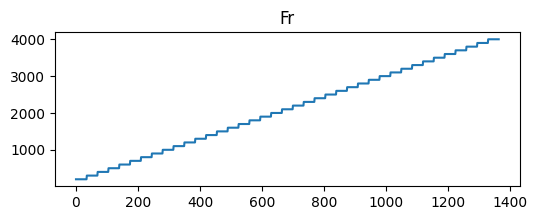
\includegraphics[scale=0.65]{assets/dataset1_column_Fr_plot.png}
	\end{figure}
	\begin{figure}
		\caption{Plot of Lifetime}
		\centering
		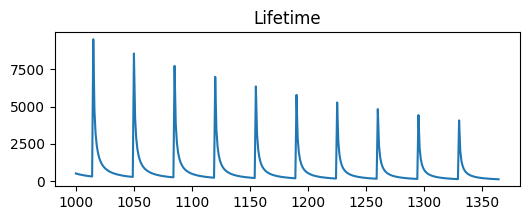
\includegraphics[scale=0.65]{assets/dataset1_column_Lifetime_plot2.png}
	\end{figure}
	\begin{figure}
		\caption{Plot of Lifetime}
		\centering
		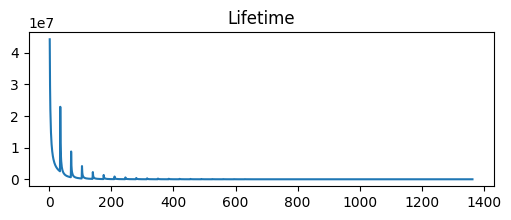
\includegraphics[scale=0.65]{assets/dataset1_column_Lifetime_plot1.png}
	\end{figure}
	\begin{figure}
		\caption{Plot of n}
		\centering
		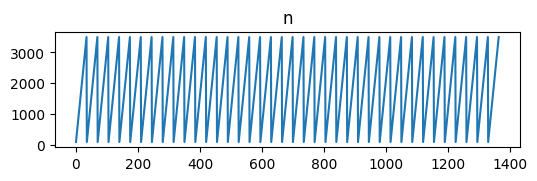
\includegraphics[scale=0.65]{assets/dataset1_column_n_plot.png}
	\end{figure}
	\begin{figure}
		\caption{Correlation matrix of dataset \#1}
		\centering
		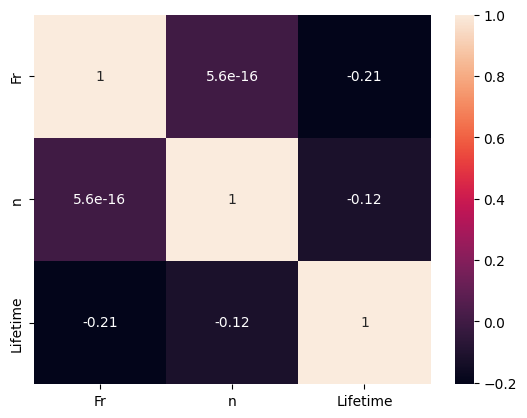
\includegraphics[scale=0.5]{assets/dataset1_correlation_matrix.png}
	\end{figure}

	\newpage
	\bibliographystyle{plain} 
	\bibliography{bibliography}
	
\end{document}